\section*{سوال ۱}

تبدیل هر FSM دلخواهی به کد Verilog یا VHDL که قابل سنتز باشد.

\section*{جواب سوال ۱}

\section*{نحوه‌ی کارکرد قفل دیجیتالی}

\noindent \textbf{ورودی‌ها}:
\begin{itemize}
	\item \lr{clk}: سیگنال ساعت
	\item \lr{rst}: سیگنال ریست
	\item \lr{inp}: سیگنال ورودی (0 یا 1)
\end{itemize}

\noindent \textbf{خروجی}:
\begin{itemize}
	\item \lr{unlocked}: این خروجی زمانی که رمز صحیح وارد شود به '1' تنظیم می‌شود.
\end{itemize}

\noindent \textbf{وضعیت‌ها}:
\begin{itemize}
	\item \lr{IDLE}: وضعیت اولیه یا زمانی که رمز نادرستی وارد شده باشد.
	\item \lr{FIRST\_BIT}: اولین بیت صحیح وارد شده است.
	\item \lr{SECOND\_BIT}: دو بیت اول صحیح وارد شده است.
	\item \lr{UNLOCKED}: وضعیت قفل باز است.
\end{itemize}

\newpage

\section*{توضیحات قفل دیجیتالی}
قفل دیجیتالی با استفاده از یک FSM طراحی شده است که رمز "101" را برای باز کردن قفل می‌پذیرد. این قفل می‌تواند در موارد زیر مورد استفاده قرار گیرد:

\begin{itemize}
	\item \textbf{واحدهای ذخیره‌سازی اطلاعات}: مانند یک فلش مموری یا یک هارد دیسک خارجی که نیاز به یک مکانیزم امنیتی ساده برای محافظت از داده‌ها دارند.
	
	\item \textbf{دستگاه‌های امنیتی}: مانند یک قفل درب الکترونیکی که با ورود یک رمز ساده باز و بسته می‌شود.
	
	\item \textbf{تجهیزات الکترونیکی}: مانند یک گجت یا یک دستگاه خاص که باید با ورود یک رمز خاص فعال یا غیرفعال شود.
	
	\item \textbf{آموزش و آزمون}: به عنوان یک مثال ساده برای آموزش مفاهیم مرتبط با FSM‌ها و طراحی مدارات دیجیتال.
\end{itemize}

به طور کلی، این قفل دیجیتال می‌تواند در هر جایی که نیاز به یک مکانیزم امنیتی ساده و الکترونیکی وجود داشته باشد، مورد استفاده قرار گیرد.

\newpage

\section*{شکل FSM برای یک قفل دیجیتالی}

در ابتدا، به دایرکتوری مورد نظر برای فعال‌سازی TrueTime در متلب مراجعه کردیم با این دستور:
\begin{figure}[h]
	\centering
	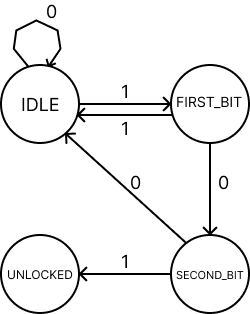
\includegraphics{1.png}
	\label{fig:label4}
\end{figure}

\newpage

\section*{کد JSON همان FSM}

\begin{figure}[h]
	\centering
	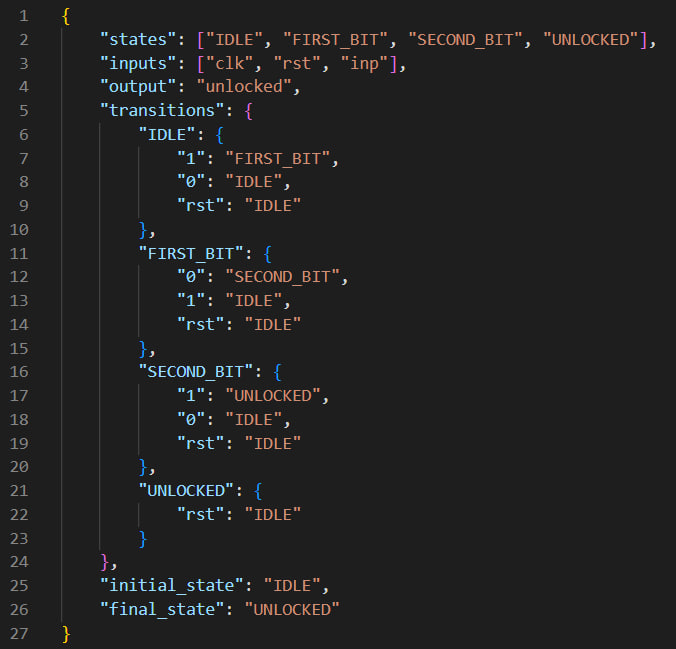
\includegraphics{2.jpg}
	\label{fig:label4}
\end{figure}

\begin{itemize}
	\item در وضعیت FIRST\_BIT اگر $inp = 1$ باشد به IDLE بر می‌گردیم.
	\item از وضعیت UNLOCKED فقط با $rst = 1$ به IDLE بر می‌گردیم.
\end{itemize}

\newpage

\section*{کد وریلاگ}

\begin{figure}[h]
	\centering
	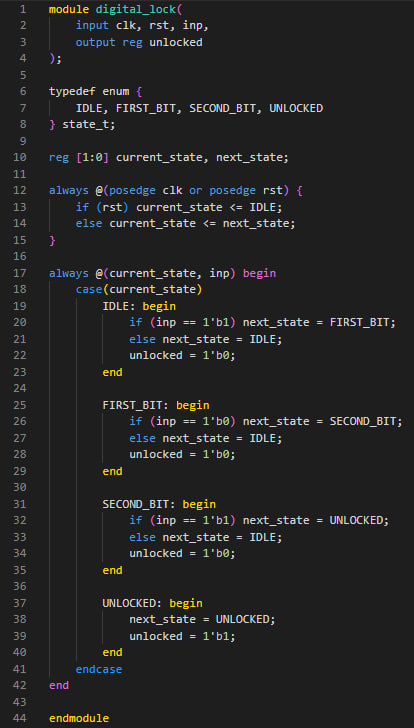
\includegraphics{3.jpg}
	\label{fig:label4}
\end{figure}

\newpage

\section*{توضیح کد وریلاگ}

\subsection*{ماژول:}
\textbf{digital\_lock}: این ماژول سه ورودی و یک خروجی دارد.

\subsection*{ورودی‌ها:}
\begin{enumerate}
	\item \textbf{clk}: سیگنال ساعت
	\item \textbf{rst}: سیگنال ریست
	\item \textbf{inp}: سیگنال ورودی که می‌تواند 0 یا 1 باشد
\end{enumerate}

\subsection*{خروجی:}

\begin{enumerate}
	\item \textbf{unlocked}: وضعیت قفل. وقتی قفل باز است، این خروجی 1 است.
\end{enumerate}

\subsection*{تعریف‌ها:}
\begin{itemize}
	\item \textbf{state\_t}:
	این enum چهار وضعیت مختلف FSM را تعریف می‌کند:
	
	IDLE , FIRST\_BIT , SECOND\_BIT و UNLOCKED.
	\item \textbf{current\_state و next\_state}: این دو متغیر وضعیت فعلی و وضعیت بعدی FSM را نگه می‌دارند.
\end{itemize}

\section*{پیاده‌سازی FSM:}
\begin{enumerate}
	\item در هر لبه مثبت clk ، \texttt{current\_state} به \texttt{next\_state} تغییر می‌کند، مگر زمانی که \texttt{rst} فعال باشد که \texttt{current\_state} به IDLE باز می‌گردد.
	\item بر اساس وضعیت فعلی و ورودی، وضعیت بعدی و خروجی تعیین می‌شوند.
\end{enumerate}

\newpage

\section*{کد پایتون Generator کد وریلاگ از هر کد json یک FSM}

\begin{figure}[H]
	\centering
	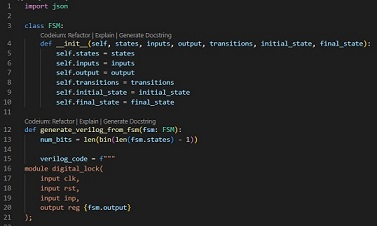
\includegraphics{4.jpg}
	\label{fig:label4}
\end{figure}

\begin{figure}[H]
	\centering
	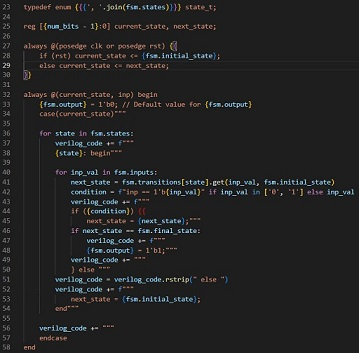
\includegraphics{5.jpg}
	\label{fig:label4}
\end{figure}

\begin{figure}[H]
	\centering
	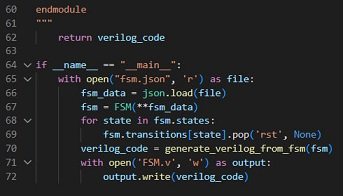
\includegraphics{6.jpg}
	\label{fig:label4}
\end{figure}

\newpage

\section*{کد پایتون Generator توضیح کد وریلاگ از هر کد json یک FSM}


کد معرفی شده، یک ماشین حالت محدود (Finite State Machine - FSM) را از یک فایل \textit{JSON} می‌خواند و بر اساس آن یک ماژول \textit{Verilog} ایجاد می‌کند.

\subsection*{کلاس FSM}

این کلاس یک ماشین حالت محدود را نمایان می‌کند. ویژگی‌های اصلی آن شامل : حالت‌ها (states) ، ورودی‌ها (inputs) ، خروجی (output) ، گذارها (transitions) ، حالت اولیه (initial\_state) و 

حالت نهایی (final\_state) است.

\subsection*{تابع generate\_verilog\_from\_fsm}

این تابع بر اساس یک شئ از نوع FSM یک ماژول Verilog ایجاد می‌کند. 

\subsection*{قسمت اجرایی}

در این بخش، فایل JSON مربوط به FSM خوانده می‌شود، و با استفاده از تابع بالا یک ماژول Verilog ایجاد و در یک فایل با نام \textit{FSM.v} ذخیره می‌شود.

\newpage

\section*{استفاده از این کد پایتون}

آن فایل json اولیه که مربوط به FSM قفل الکترونیک بود را به عنوان ورودی به این کد می‌دهیم و خروجی، کد وریلاگی‌ست که می‌خواهیم.